% Copyright (c) 2021 Eclipse Arrowhead Project
%
% This program and the accompanying materials are made available under the
% terms of the Eclipse Public License 2.0 which is available at
% http://www.eclipse.org/legal/epl-2.0.
%
% SPDX-License-Identifier: EPL-2.0

For a document, \GlossaryHyperRef{model}{model}, or other \GlossaryHyperRef{artifact}{artifact}, to be allowed to claim conformance to this document, the following must be observed by that \textit{derived work}:

\begin{enumerate}
\item At least one of the concepts defined in this work must be part of that derived work.
\item The derived work must make it explicit what concepts are taken from this work.
	\begin{enumerate}
	\item How this is done most suitably depends on the type of derived work. A document may include a normative reference to this document, while a model may want to give all relevant \GlossaryHyperRef{entity}{entities} and \GlossaryHyperRef{relationship}{relationships} an \GlossaryHyperRef{attribute}{attribute} with the identity of this document, for example.
	\end{enumerate}
\item Every concept taken from this work must be represented by the name it is given here.
	\begin{enumerate}
	\item If important to be able to distinguish an Arrowhead concept from other such of relevance, concepts from this work may be qualified by the leading word ``Arrowhead'', as in, for example, ``Arrowhead system`` or ``Arrowhead service function''.
	\item Note that some concepts defined here are given more than one name. For example, \GlossaryHyperRef{function-program}{program function} and \GlossaryHyperRef{procedure-software}{software procedure} are declared to be synonyms in the glossary. When synonyms exist, only one of their entries in the glossary will have a definition. The name of that definition should be the name being used.
	\end{enumerate}
\item Concepts taken from this work may be \textit{specialized} and/or \textit{simplified}, but must never be \textit{contradicted}.
	\begin{enumerate}
	\item \textit{Specialization} means that more \GlossaryHyperRef{constraint}{constraints} are applied to it than are presented here. For example, a certain derived work may require that all devices have \GlossaryHyperRef{unit-compute}{compute units} supporting a certain instruction set, or that every \GlossaryHyperRef{system}{system} \GlossaryHyperRef{provider-service}{provides} a specific monitoring \GlossaryHyperRef{service}{service}, and so on.
	\item \textit{Simplification} means that entities, relationships or attributes introduced here are omitted due to being outside the scope of the derived work. For example, a technical document may not be concerned with \GlossaryHyperRef{role-stakeholder}{stakeholder roles}, while a model of certain types of local clouds may not be concerned with whether or not artifacts are \GlossaryHyperRef{resource}{resources} or not, and so on.
	\item \textit{Contradiction} means that an attribute or other constraint is introduced that makes it impossible to reconcile the concepts presented here with those in the derived work. A derived work must not, for example, demand that no devices ever host systems. Contradictions generally only occur when some relationship or attribute is both demanded to exist and not to exist at the same time.
	\end{enumerate}
\item If a different graph notation is used than the one described in Section \ref{sec:introduction:conventions:graphs}, the derived work must either describe how its notation maps to the notation here, or refer to a work making such a description.
	\begin{enumerate}
	\item The graph constructs that have to be mapped are as follows:
		\begin{enumerate}
		\item \textit{entities}, which are the boxes with solid lines and names inside them;
		\item \textit{relationships}, which are the unidirectional arrows denoting relationships;
		\item \textit{attributes}, which are the \textit{names} and \textit{quantifiers} associated with graph relationships;
		\item \textit{groups}, which are the boxed dashed lines that encapsulate entities and other groups;
		\item \textit{combined relationships}, which are relationships with a shared target or source end; and
		\item \textit{custom attributes}, which are special attributes expressed in text only.
		\end{enumerate}
		Mapping to the latter three constructs must be specified only if they are used by concepts of relevance to the derived work. Most uses of combined relationships in this work can be substituted for many regular relationships without loss of information. If only such combined relationships are of relevance to a derived work, that work may choose to not include a mapping to the combined relationship construct. Each relevant type custom attribute of this work must receive its own individual mapping.
	\item In practice, only text documents claiming to adhere to the graph diagram notation of Section \ref{sec:introduction:conventions:graphs} are exempt from having to describe or refer to such a notational mapping. As mappings to this document will be hard to produce rigorously without text, we expect all such mappings to be described in text documents.
	\end{enumerate}
\end{enumerate}

\subsection{ISO/IEC/IEEE 42010}
\label{sec:conformance:iso42010}

The ISO42010 \cite{iso42010} standard provides a uniform way for system architects to produce architectural \GlossaryHyperRef{description}{descriptions}, \GlossaryHyperRef{viewpoint-architecture}{viewpoints}, \GlossaryHyperRef{framework-architecture}{frameworks} and \GlossaryHyperRef{language-architecture-description}{description languages}.
In the context of ISO42010, this work can be used as a \GlossaryHyperRef{metamodel}{\textit{metamodel}} part of an architectural viewpoint, as illustrated in Figure \ref{fig:iso42010}.

\begin{figure}[ht!]
  \centering
  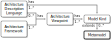
\includegraphics[scale=0.9]{figures/iso42010}
  \caption{
    The metamodel as a part of an ISO42010 architectural viewpoint.
  }
  \label{fig:iso42010}
\end{figure}